\documentclass[border=8pt]{standalone}
\usepackage{tikz}
\usetikzlibrary{positioning,arrows.meta,shapes.geometric,fit,calc}
\usepackage[T1]{fontenc}
\usepackage{helvet}
\renewcommand{\familydefault}{\sfdefault}

\definecolor{inputblue}{HTML}{3B82F6}
\definecolor{stagegreen}{HTML}{10B981}
\definecolor{reasonviolet}{HTML}{8B5CF6}
\definecolor{outputorange}{HTML}{F59E0B}

\begin{document}
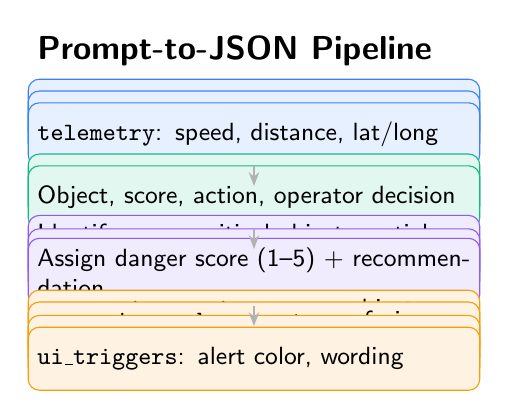
\begin{tikzpicture}[
    node distance=0.5cm,
    every node/.style={font=\small},
    stage/.style={rectangle, rounded corners=4pt, draw=#1, fill=#1!12,
                  text width=5.5cm, minimum height=0.8cm, align=left,
                  font=\small, text=black},
    header/.style={font=\small\bfseries, text=#1},
    arrow/.style={-{Stealth[length=5pt]}, thick, color=gray!60},
]

% Title
\node[font=\large\bfseries, text=black] (title) {Prompt-to-JSON Pipeline};

% Input packaging
\node[header=inputblue, below=0.6cm of title, anchor=west] (h1) at (title.west |- {0,0}) {\textsc{1. Modality Packaging}};
\node[stage=inputblue, below=0.15cm of h1.west, anchor=west] (s1a) {\texttt{image}: base64-encoded frame};
\node[stage=inputblue, below=0.15cm of s1a.west, anchor=west] (s1b) {\texttt{audio}: base64-encoded clip (optional)};
\node[stage=inputblue, below=0.15cm of s1b.west, anchor=west] (s1c) {\texttt{telemetry}: speed, distance, lat/long};

% History injection
\node[header=stagegreen, below=0.5cm of s1c.west, anchor=west] (h2) {\textsc{2. Recent-History Injection}};
\node[stage=stagegreen, below=0.15cm of h2.west, anchor=west] (s2a) {Up to 15 prior incident summaries};
\node[stage=stagegreen, below=0.15cm of s2a.west, anchor=west] (s2b) {Object, score, action, operator decision};

% Reasoning instructions
\node[header=reasonviolet, below=0.5cm of s2b.west, anchor=west] (h3) {\textsc{3. Staged Reasoning Instructions}};
\node[stage=reasonviolet, below=0.15cm of h3.west, anchor=west] (s3a) {Identify scene, critical object, spatial cues};
\node[stage=reasonviolet, below=0.15cm of s3a.west, anchor=west] (s3b) {Compare visual vs.\ telemetry vs.\ audio};
\node[stage=reasonviolet, below=0.15cm of s3b.west, anchor=west] (s3c) {Assign danger score (1--5) + recommendation};

% Output schema
\node[header=outputorange, below=0.5cm of s3c.west, anchor=west] (h4) {\textsc{4. Constrained JSON Response}};
\node[stage=outputorange, below=0.15cm of h4.west, anchor=west] (s4a) {\texttt{perception\_engine}: scene, object, kinetics};
\node[stage=outputorange, below=0.15cm of s4a.west, anchor=west] (s4b) {\texttt{reasoning\_and\_commentary}: fusion notes};
\node[stage=outputorange, below=0.15cm of s4b.west, anchor=west] (s4c) {\texttt{action\_policy}: score, action, report};
\node[stage=outputorange, below=0.15cm of s4c.west, anchor=west] (s4d) {\texttt{ui\_triggers}: alert color, wording};

% Arrows between sections
\draw[arrow] (s1c.south) -- ++(0,-0.25);
\draw[arrow] (s2b.south) -- ++(0,-0.25);
\draw[arrow] (s3c.south) -- ++(0,-0.25);

\end{tikzpicture}
\end{document}
